\documentclass[12pt]{article}

% Language setting
% Replace `english' with e.g. `spanish' to change the document language
\usepackage[english]{babel}

% Set page size and margins
% Replace `letterpaper' with `a4paper' for UK/EU standard size
\usepackage[a4paper,top=2.4cm,bottom=2.4cm,left=2.4cm,right=2.4cm,marginparwidth=1.75cm]{geometry}

% Useful packages
\usepackage{amsmath}
\usepackage{graphicx}
\usepackage[colorlinks=true, allcolors=blue]{hyperref}
\usepackage[printonlyused,withpage]{acronym}
\usepackage[version=4,arrows=pgf-filled]{mhchem}
\usepackage{float}
\usepackage{booktabs}

\usepackage{pgfplots}
\pgfplotsset{compat=1.18}
% Set global legend style
\pgfplotsset{
    every axis legend/.append style={
        draw=none % Remove legend border
    }
}
\usepgfplotslibrary{dateplot}
\usetikzlibrary{pgfplots.dateplot,}

\usepackage{multirow, multicol}
\usepackage{cleveref}
\usepackage{numprint}
\npthousandsep{,}

% packages for table
\usepackage{siunitx}
\usepackage{array}
\usepackage{booktabs}
\usepackage{csvsimple}
\usepackage{multirow}

%package for indent
\usepackage{indentfirst}
\setlength{\parindent}{1cm}% too much in my eyes delete this
                             % line and use the default ...


\counterwithin{figure}{section}
\counterwithin{table}{section}
\linespread{1.5}
\begin{document}

\pagenumbering{gobble}% Remove page number
\begin{titlepage}
\begin{figure}[H]
\centering
\includegraphics[width=0.5\linewidth]{logo.png}
\end{figure}


   \begin{center}
       \vspace*{1cm}

       MS 4015 – Industrial Research

       \vspace{0.5cm}
        {\fontsize{20}{24}\selectfont \textbf{Performance Evaluation of Wastewater Treatment Plant Moratuwa/Ratmalana}}
            
       \vspace{1.5cm}

       April, 2024

       \vfill
            
      A report submitted in partial fulfillment of the requirement for the Internship \\
       Training of the Faculty of Science, University of Colombo
            
       \vspace{0.8cm}
            
       \textbf{U. G. K. Perera}\\
       2019s17442\\
       s14968\\
       
            
   \end{center}
\end{titlepage}


\pagenumbering{roman}

\newpage
\section*{\centering Declaration}
\addcontentsline{toc}{section}{Declaration}

  \vspace{0.5cm}

I, U. G. K. Perera, a senior student at the Faculty of Science, University of Colombo, affirm that this research report, named "Performance Evaluation of Wastewater Treatment Plant Moratuwa/Ratmalana is entirely my work. The research was conducted under the guidance of Mrs. T.A.D.A.E. Jayathilake, the chemist at the Moratuwa/Ratmalana Wastewater Treatment Plant, and supervised by Dr. Ayomi Withrana, a senior lecturer in the Department of Zoology and Environmental Sciences at the University of Colombo. All extra assistance received has been properly acknowledged in the report. The paper includes proper citations and references for all sources accessed. This report has not been previously submitted for evaluation, either in its entirety or in part, at this institution or any other.

  \vspace{2cm}

 


 \hspace*{\fill} \includegraphics[height=3cm]{assets/sign_gavini.png} \\
 \hspace{0.5cm} $20^{th}$ March, 2024  \hspace*{\fill} \textit{Signature of Student}\\

  \vspace{0.5cm}

  \hspace*{\fill} \includegraphics[height=1.5cm]{assets/sign_placement_mentor.png} \\
  \hspace{1cm} $29^{th}$ March, 2024 \hspace*{\fill} \textit{Signature of Placement Mentor}\\

  \hspace*{\fill}  \\
  \hspace{1cm} \  April, 2024 \hspace*{\fill} \textit{Signature of Academic Mentor}  \\


\clearpage

\newpage
\section*{\centering Acknowledgements}
\addcontentsline{toc}{section}{Acknowledgements}

I sincerely thank the following people and institutions for assisting me in finishing this study report.

First and foremost, I extend my heartfelt thanks to my placement mentor, T.A.D.A.E Jayathilake, the Chemist at the Wastewater Treatment Plant Moratuwa/ Ratmalana, for her invaluable guidance and unwavering support throughout the duration of my placement.

I am also deeply grateful to my academic mentor, Dr. Ayomi Witharana, Senior Lecturer of Zoology and Environmental Sciences, for insightful advice, encouragement, and constructive feedback which have greatly enriched the quality of this research.

I extend my appreciation to the National Water and Drainage Board for providing access to essential data and resources relevant to this study. Furthermore, I would like to express my gratitude to the staff members, especially the lab assistant and technicians of the Wastewater Treatment Plant, Moratuwa/ Ratmalana who provided valuable information about the plant operations.

Also, I would like to express my gratitude to my brother, U.A.C Perera, and my friend, W.M.S.H Warnasooriya for assisting me in producing the final report and motivating me to successfully finish the project.

Finally, I would like to thank my family and my university colleagues for their unwavering support, understanding, and encouragement throughout this journey. Their love and encouragement have been my constant source of strength.

This research would not have been possible without the collective support and encouragement of all those mentioned above. Thank you for being a part of this journey and for your invaluable contributions.

\clearpage

\newpage
\section*{\centering Executive Summary}
\addcontentsline{toc}{section}{Excecutive Summary}


This study aims to assess the performance evaluation of a \ac{WWTP} located at Moratuwa/ Ratmalana during a selected period in 2023. Data were collected based on the physiochemical parameters such as pH and temperature, as well as chemical parameters including \ac{BOD}, \ac{COD}, \ac{TSS}, \ac{OG}, Ortho-Phosphate (Dissolved Phosphate), and Fluoride from the inlet and outlet. Under sludge management, sludge samples were collected from the sludge storage tank, return water and dewatered sludge samples from the belt press and the dried sludge samples from the drying bed to test for the \ac{TSS}, moisture content, solid content, and \ac{SVMC}.

This study was conducted to accomplish several objectives, such as evaluate the effluent quality based on the standards issued by \ac{CEA}, Sri Lanka, evaluate the efficiencies of removing contaminants through the biological treatment process, evaluate the belt press efficiency and analysis of the sludge drying process and moisture removal percentage.

The performance evaluation presents the following removal efficiencies; 93.55\% of \ac{BOD}, 86.95\% of \ac{COD}, 95.28\% of \ac{TSS}, 97.04\% of \ac{OG}, 79.08\% of ortho-phosphate, and 68.04\% of Fluoride.  This study also investigated the efficiency of the belt press dewatering process under two criteria and the moisture removal percentages during the drying period.  It was revealed that the study findings can be used to identify and fix operating and maintenance issues and plan future plant expansions to accommodate higher hydraulic and organic loads.


\newpage
\tableofcontents

\newpage
\listoffigures
\section*{}
\addcontentsline{toc}{section}{List of Figures}

\newpage
\listoftables
\section*{}
\addcontentsline{toc}{section}{List of Tables}

\newpage
\section*{Abbreviations}
\addcontentsline{toc}{section}{Abbreviations}
\begin{acronym}\itemsep=-20pt

\acro{BOD}{Biochemical Oxygen Demand}
\acro{COD}{Chemical Oxygen Demand}
\acro{TSS}{Total Suspended Solids}
\acro{SVMC}{Sludge Volatile Matter Content}
\acro{MLVSS}{Mixed Liquor Volatile Suspended Solids}
\acro{WWTP}{Wastewater Treatment Plant}
\acro{OG}[O\&G]{Oil and Grease}
\acro{NWSDB}[NWS\&DB]{National Water Supply and Drainage Board}
\acro{F/M Ratio}{Food to Mass Ratio}
\acro{BOD5}[BOD$_5$]{Biochemical oxygen demand in 5 days}
\acro{TS}{Total Solids}
\acro{DO}{Dissolved Oxygen}
\acro{SV30}[SV$_{30}$]{Settleable Volume in 30 minutes}
\acro{SVI}{Sludge Volume Index}
\acro{TDS}{Total Dissolved Solids}
\acro{MLSS}{Mixed Liquor Suspended Solids}
\acro{TS} {Total Solids} 
\acro{CEA}{Central Environmental Authority}
\end{acronym}

\newpage
\pagenumbering{arabic}
\section{INTRODUCTION}
Water is a fundamental requirement for all living organisms and is one of the most important resources on earth \cite{Smarzewska2021}. The rapid population growth has impacted resource utilization and led to water pollution. Wastewater consists of both liquid and solid waste generated by residential properties,
commercials and agriculture-related activities, as well as any other kind of water used by humans that is subsequently released into a sewerage system
with poor quality \cite{Prasad2020}.

Domestic wastewater can be categorized into two types, and they are greywater and blackwater. Greywater is the wastewater generated from bathtubs, laundry machines, hand basins, showers, and kitchen sinks, excluding any input from toilets. Approximately 75\% of the total household sewage is composed of greywater \cite{Eriksson2002}. Blackwater originates from toilets and contains water, urine, excrement, and toilet paper materials \cite{Paulo2013}. The composition of contaminants in wastewater may fluctuate depending on the specific industrial,
agricultural and municipal activities that discharge them. The pollutants are classified into three categories: inorganic, organic, and biological \cite{Sangeetha2023}.

The composition of the wastewater can result in adverse impacts on the environment, aquatic and wildlife populations and could potentially contaminate drinking water sources \cite{Smarzewska2021}. Organic matter can lead to oxygen depletion in rivers, lakes, and streams. Eventually, the biological decomposition of organic matter may lead to fish mortality and unpleasant smells. Also, wastewater includes nutrients that might enhance the growth of aquatic plants and may contain toxic substances that could be carcinogenic or mutagenic \cite{Prasad2020}. Therefore, wastewater treatment is essential before discharge to the water bodies.

Wastewater treatment involves separating and breaking down some of the solids that are in wastewater and turning complex organic compounds into minerals or relatively stable organic solids \cite{Sonune2004}. There are several \ac{WWTP}s that are operated under the \ac{NWSDB} in Sri Lanka, located in Moratuwa/Ratmalana, Kandy, Kurunegala, Jaela/Ekala, Seethawake, Katharagama, etc. These plants use different types of treatment processes, such as aerated lagoons, activated sludge treatment, and oxidation ditches. The activated sludge treatment process is a common technique used to treat wastewater, including municipal sewage and industrial wastewater \cite{AGUILAR2013, Chukwu2018}. Treated water from these \ac{WWTP}s' is discharged by a short sea outfall (600 m away from the seashore) and to the surface water in Sri Lanka.

\begin{sloppypar}
Sludge is identified as a solid by-product of biological wastewater treatment that contains harmful substances such as heavy metals, pathogens, and organic contaminants \cite{Wu2020}, and the wet sludge can contain up to 98\% of water content
\cite{Chan2016, SyedHassan2017}. Sewage sludge production has increased globally due to rising population, industrialization, and urbanization, and the characteristics of the sludge vary with the source of the wastewater. Dewatering and drying are important procedures to reduce the volume for easy transportation and further sludge treatment \cite{Chang2023}. 
\end{sloppypar}

With reference to the \Cref{fig:Sludge_water}, the water content can be classified as (i) free (or bulk), (ii) vicinal (or surface), (iii) interstitial, and (iv) chemically bound (or hydration) based on the interaction with sludge solid particles \cite{SyedHassan2017, Qi2020, Vaxelaire2004, Novak2006}. Free water, which can be eliminated through drainage, mechanical dewatering, or thickening, refers to water that is not connected to or affected by the suspended solid particles. It is the most readily removable water from the wet sludge. Interstitial water is confined within the fissures and interstitial spaces of the flocs and organisms.


\begin{figure}[H]
\centering
\fbox{\includegraphics[width=.75\textwidth]{moisture distribution.jpg}}
\caption{Classification of water in sewage sludge}\cite{Qi2020}
\label{fig:Sludge_water}
\end{figure}

Interstitial water can be transitioned into free water when the flocs and microbial cells are eliminated. Applying mechanical energy can remove a significant amount of water by pressing it out of the sludge. Many dewatering techniques can remove both interstitial and bulk water from the sludge, and dewatered sewage sludge typically includes 73–84\% moisture \cite{Chan2016}.
 
Sewage sludge management is financially and environmentally complex due to social challenges, high treatment expenses, health risks, and limited sustainable disposal methods \cite{Fuerhacker2011}. Some disposal methods for sludge are as fertilizers, some as fuel, and some as raw materials for building materials \cite{Bratina2016}.
 
Evaluating the performance of a treatment plant involves measuring its efficiency using known indicators such as the removal of pollutants such as \ac{BOD}, \ac{COD}, and suspended solid contaminants. Operational difficulties can be detected through these evaluations and may be fixed to ensure that the plant functions properly \cite{Khan2018}. The performance efficiency of a treatment plant relies not only on its correct design and construction but also on proper operation and maintenance \cite{Kumar2010}.

 
Therefore, this study was designed to evaluate the performance of \ac{WWTP} and sludge management.


The objectives are to; 
 
 (1) evaluate the effluent quality based on the standards. 
 
 (2) analyze the removal efficiencies of the contaminants through the biological treatment.
 
 (3) analyze the sludge dewatering and drying processes.

\newpage
\section{MATERIALS AND METHODS}

\subsection{Overview of the Treatment Plant}

The \ac{WWTP} located at Moratuwa/ Ratmalana was chosen as the study location for this study. It was established in 2013 under the \ac{NWSDB} of Sri Lanka. It has been designed with a total capacity of 17,000 \unit{m^3}/day. Four pumping stations located at Badowita, Ratmalana, and Thelawala supply wastewater from 5,700 domestic and 239 industrial connections directly to this plant, and 510 \unit{m^3}/day (3\% of the total capacity) supplied by gully bowsers.

The Moratuwa/ Ratmalana Treatment Plant is a biological treatment Plant that uses the activated sludge method to treat wastewater. The biological basin has been designed using the reverse A2O system. This is the first-ever reverse A2O Plant in Sri Lanka \cite{Danushika2016}. There are Primary, Secondary, and Tertiary treatment processes at this premises. 

\begin{figure}[H]
\centering
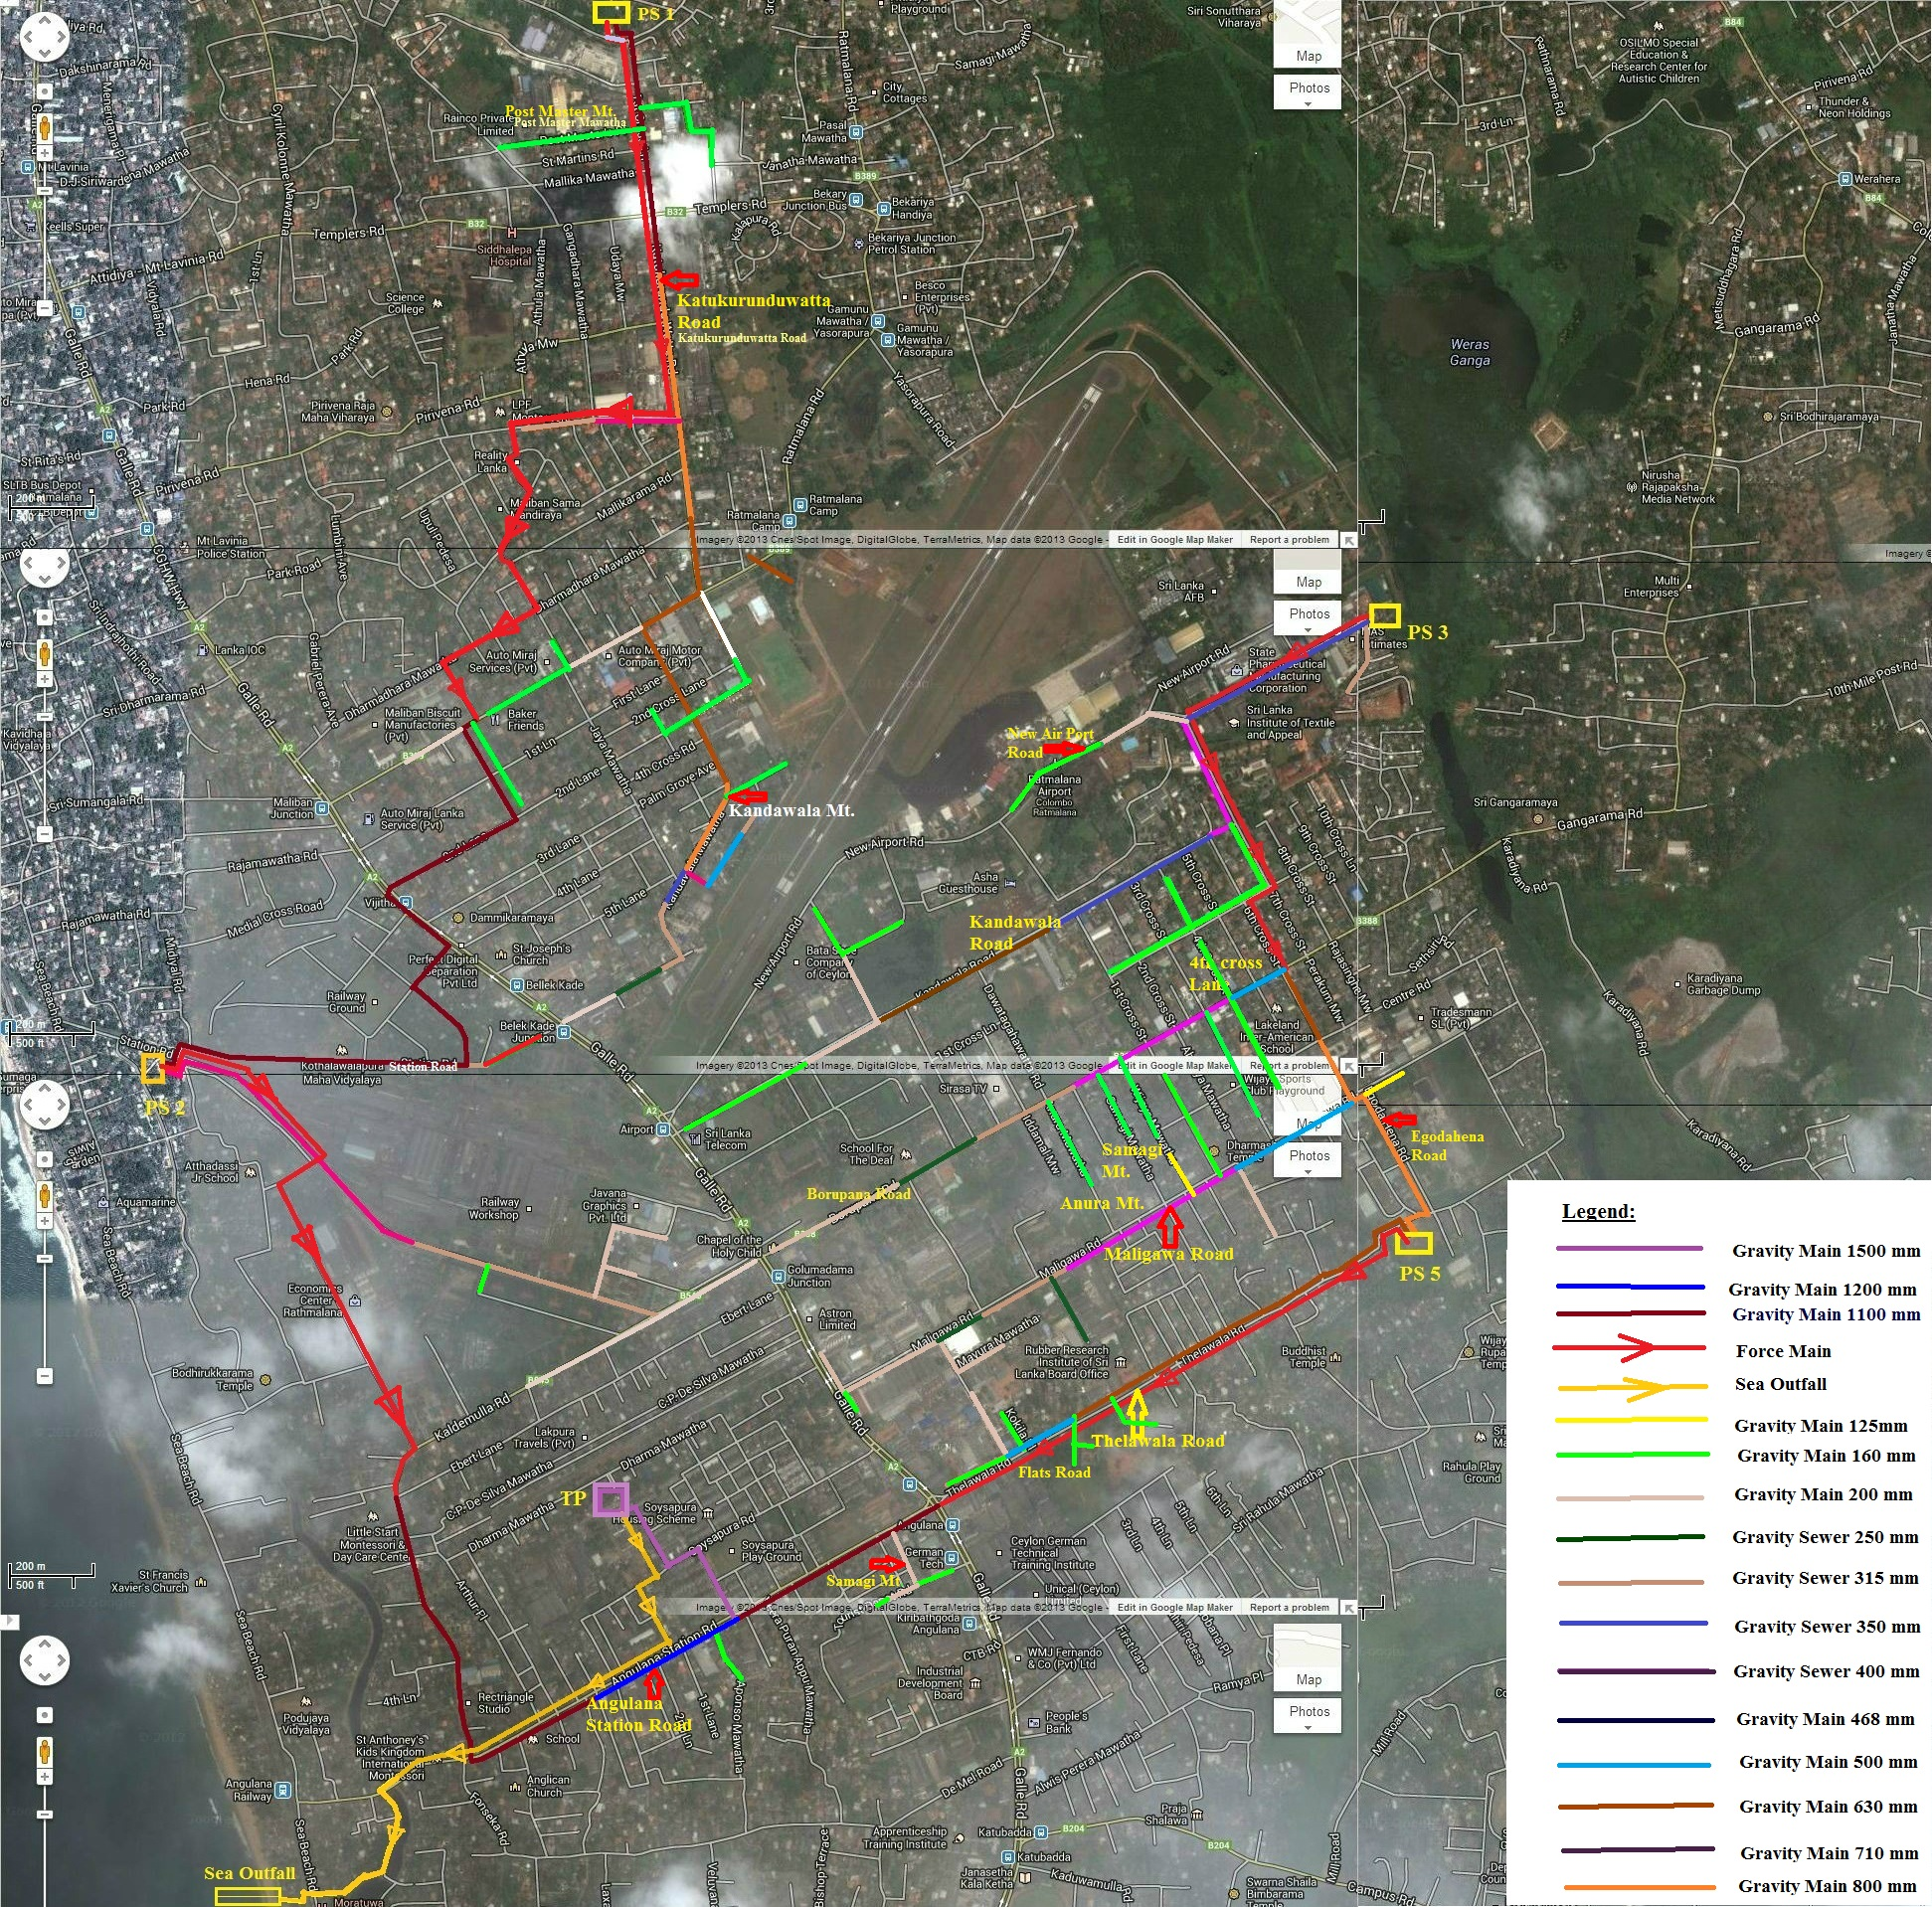
\includegraphics[width=0.756\linewidth]{connection_network_map.png}
\caption{Connection network map; source: \ac{NWSDB}}
\label{fig:connection_network_map}
\end{figure}



\subsubsection{Primary Treatment}
Wastewater arrived at the collecting chamber by gravity from 4 pumping stations and from the septic sludge receiver, which unloaded the gully. Collected wastewater in the inlet chamber goes through the coarse screen that has free slots of 40 mm between the bars to remove large matter from the wastewater. After the coarse screening, the flow arrives at the inlet well and is pumped to the fine screen by an inlet pumping station equipped with three submersible pumps. Pumped wastewater goes through a fine screen that has free slots of 3 mm between the bars to remove small particles. The screened water arrives at the grit traps to settle and remove the sand and heavy particles. Pretreated water is collected in the collecting chamber, and there is a bypass to control the overflow higher than the design flow. Before the secondary treatment, the split box is fixed to divide the flow into two streams.

\subsubsection{Secondary Treatment/ Biological Treatment}
Biological treatment started in the denitrification basin, and 60\% of the influent flow arrived at the basin that was divided by the split box, mixed with the return-activated sludge recirculated from the clarifiers. There is low dissolved oxygen content, but the oxygen that is bound with nitrogen as nitrate is available in the flow. Therefore, these denitrification basins have anoxic conditions, and denitrification occurs under these conditions.


For better denitrification, it is necessary to keep the oxygen concentration in the basin below 0.5 \unit{mg/l}. There is a 2.8 \unit{hour} retention time in the anoxic basin. After denitrification, water arrives at the anaerobic basin and is mixed with 40\% of the influent flow divided by the split box. Anaerobic basin doesn't have a concentration of dissolved Oxygen, and under this anaerobic condition, phosphorous-accumulating microorganisms store organic materials and release the phosphorous. Untreated influent that arrives from the split box ensures the availability of easily biodegradable organic matter. There is a 1.3 \unit{hour} retention time in the anaerobic basin.

After the anaerobic basin, water arrives at the aerobic basin for nitrification. Here, microorganisms metabolize organic matter by consuming Oxygen and releasing Carbon dioxide and water. Microorganisms use organic matter and nutrients as an energy source for growth. In an anaerobic tank, nitrification is prominent under a dissolved Oxygen concentration range of 1.5 - 2.0 \unit{mg/l} and occurs as per the following formula.
\begin{gather}
    \ce{NH4^+ + 2 O2 -> NO3-  + H2O  + 2 H+ }
\end{gather}

The fine bubbler rubber membrane diffusers are installed at the bottom of the basin to distribute the air, and the oxygen concentration is controlled by oxygen meters. All these three basins are equipped with submersible mixtures to obtain complete contact with the wastewater and the sludge and avoid settling the sludge. There is a 9.9 \unit{hour} retention time in the aerobic basin.

\begin{figure}[H]
\centering
\includegraphics[width=1\linewidth]{material_and_methodology/Biological Treatment basins.JPG}
\caption{Biological treatment basins}
\label{fig:Biological_treatment_basins}
\end{figure}

After the biological treatment, the treated water arrives at the sedimentation tank for clarification. In the sedimentation tank, gravitational forces separate the activated sludge flocks from the treated water. The travelling Bridge Siphon Scraper is installed at the sedimental tank to lift the sludge from the bottom of the sedimentation tank to a longitudinal sludge channel by siphon action. Once the biological treatment is completed, the treated wastewater is led to the treated water channel. There is a 6.9 \unit{hour} retention flow through the clarifiers.

\begin{figure}[H]
\centering
\includegraphics[width=1\linewidth]{material_and_methodology/Sedimentation basin.jpg}
\caption{Sedimentation tank}
\label{fig:Sedimentation_tank}
\end{figure}
\subsubsection{Chemical Treatment}
Sodium Hypochlorite is used in the chlorination unit to disinfect the treated wastewater. The hypochlorite is dosed at the outlet flow in case of epidemic diseases in circulation. The treated wastewater was discharged by a short sea outfall in the Angulana area.  

\subsubsection{Compost Filter}
Ventilation air collected from septic sludge handling, Screen washers, screening containers, sand separators, and grit containers is transported by a fan to a compost filter for odour reduction. Compost filters are filled with small pieces of coconut husk to grow the microorganism. The treated wastewater is sprayed into the tank to protect the coconut husk's moisture content and ensure the microorganisms' growth. 

\begin{figure}[H]
\centering
\includegraphics[width=1\linewidth]{material_and_methodology/diagram_of_treatment_plant.png}
\caption{Schematic Diagram of the wastewater treatment plant.}
\label{fig:treatment_plant}
\end{figure}

\subsubsection{Sludge Treatment}
If the suspended Solid concentration in the return sludge channel is higher than the limit, the excess sludge is withdrawn from the return sludge flow. The sludge flow arrives at either one of two sludge storage tanks. The sludge storage tanks have submersible mixers to avoid sedimentation during dewatering, and from the storage tank, the sludge is pumped to the belt filter press for dewatering. Before dewatering sludge, the digested sludge is typically treated to create flocs that can be easily filtered \cite{Chen2002}. Therefore, a polymer solution (cationic polyacrylamide) is dosed into the sludge flow. Belt filter presses typically include two or, in some instances, three filtering belts that converge to create a closed envelope shape. The flocculated sludge is first dewatered by gravity and then compressed between two belts. Filtration takes place in the gravity drainage zone without applying pressure to the sludge. The sludge solids percentage is typically between 6\% and 10\% after water drainage. Subsequently, as pressure rises, water trapped inside and between sludge particles is expelled \cite{Mamais2009}. The sludge flow to the belt press is measured with a flow meter, and the dewatered sludge is carried from a belt filter press to the truck using a screw conveyor and transported to the drying bed.

\begin{figure}[H]
\centering
\includegraphics[width=1\linewidth]{material_and_methodology/Belt press.jpg}
\caption{Belt Filter Press}
\label{fig:Belt_filter_press}
\end{figure}

\begin{figure}[H]
\centering
\includegraphics[width=1\linewidth]{material_and_methodology/Beltpress feeding area.JPG}
\caption{Belt Filter Press feeding area}
\label{fig:Beltpress_Feeding_area}
\end{figure}

There are 5 large and 10 small fans equipped at the drying bed that work 24 hours to decrease the inside humidity. There is a large fan that draws out the inside air. There is a rotary that activates hourly for thinning sludge.

\begin{figure}[H]
\centering
\includegraphics[width=1\linewidth]{material_and_methodology/Sludge Drying bed.jpg}


\caption{Sludge drying bed}
\label{fig:Sludge_Drying_Bed}
\end{figure}

\subsection{Sample Collection}

\subsubsection{Wastewater Sampling Points}
The performance study of wastewater treatment is done using experimental data obtained from the laboratory at the \ac{WWTP} in Moratuwa/Ratmalana. The quality of inlet and outlet wastewater was tested on a daily and weekly basis in the laboratory. pH, temperature, \ac{TDS}, \ac{DO}, and color at inlet and outlet wastewater, as well as \ac{SV30} and \ac{DO} levels of the aerobic tank, were tested daily as operational parameters. Also, pH, temperature, \ac{TDS}, \ac{TSS}, \ac{OG} concentration, fluoride, \ce{NO3-} (As N), \ce{PO4-} (As P), \ac{DO}, color at the inlet and outlet wastewater, and \ac{MLSS}, \ac{MLVSS}, \ac{F/M Ratio}, \ac{TS}, \ac{DO}, \ac{SV30}, and \ac{SVI} in the aerobic tank were tested weekly as verification parameters.

This performance evaluation has been conducted through the process of comparison. The data collection process involved gathering information over a period of 30 weeks from both the inlet and outlet of the treatment plant. The collected data parameters were inlet flow, pH, temperature, \ac{BOD5}, \ac{COD}, \ac{TSS}, fluoride, \ce{PO4-} (As P), and \ac{OG}. Each week included one data set for each parameter of the inlet and outlet, and during this evaluation, each sample was renamed with a unique sample number, as mentioned in \cref{table:sample_numbering}.  In the last 5 weeks of the data collection period, I actively worked with the lab assistant to test the parameters. All the tests related to the collected data have been done according to the procedures outlined in the Standard Methods for the Examination of Water and Wastewater \cite{APHA}.


\begin{figure}[H]
\centering
\includegraphics[width=1\linewidth]{material_and_methodology/sample_point_inlet_outlet.png}


\caption{Inlet and outlet sampling points}
\label{fig:sample_points_inlet_outlet}
\end{figure}



\subsubsection{Sludge Sampling Points}
The samples were collected from three locations, and the analyzed parameters and number of samples from December to February are shown below:

\begin{table}[H]
\caption{Sample details related to the sludge}
\centering
\begin{tabular}{|>{\centering\arraybackslash}p{1.5cm}|l|l|>{\centering\arraybackslash}p{2cm}|l|}
\hline
Sample Name & Sample Location & Sample Description & Number of Samples & Tested Parameters \\
\hline
$S_1$ & Sludge storage tank & Thickened sludge & 1 & TSS \\
\hline
$S_2$ & Dewatered unit & Reject water & 1 & TSS \\
\hline
$S_3$ & Dewatered unit & Dewatered sludge & 3 & Moisture content \\
\hline
$S_4$  & Sludge drying bed & Dried sludge & 15 & Moisture content \\
\hline
\end{tabular}

\label{table:sample_details}
\end{table}

Three $S_4$ samples mentioned in \cref{table:sample_details} were collected from three sampling points in a line, as shown in \cref{fig:samples_collected_points}, to analyze the moisture content of dried sludge, and 10 mg of each sample was mixed and one sample named as $S_5$ was prepared. The remaining four samples ($S_5$) were prepared  in the same manner using other $S_4$ samples.

\begin{figure}[H]
\centering
\includegraphics[width=1\linewidth]{material_and_methodology/sample_collected_point_dryingbed.png}
\caption{Samples collected points in the drying bed}
\label{fig:samples_collected_points}
\end{figure}


\subsection{Determination of Total Suspended Solid}
Two dry and clean glass microfiber filter papers with watch glasses were weighed, and sample $S_1$ and sample $S_2$ mentioned in \cref{table:sample_details} were filtered using pre-weighed glass microfiber filter papers. Each piece of filtered paper was kept on the watch glass and stored at 105 ℃ for 1 hour. After 1 hour, samples were removed and placed in a desiccator until they reached a constant weight. Then, samples were weighted, and \ac{TSS} was calculated using the below formula:

\begin{equation}
    \text{TSS} = \dfrac{\text{Weight of suspended solid (\unit{mg})}}{\text{Volume of water filtered (\unit{l})}}
\end{equation}

\subsection{Determination of Moisture Content}
Dry and clean aluminum foil containers were weighted, and used to tare the balance. Three samples of $S_3$ mentioned in \cref{table:sample_details} and five samples of $S_5$  were added to each container and measured for weight. Then, the samples were stored at 105 °C for 18 hours. After 18 hours, samples were removed and placed in a desiccator until they reached a constant weight. Then, samples were weighted, and moisture content was calculated using the below formula:

\begin{equation}
    \text{Moisture Content} = \dfrac{\text{Wet weight of sludge (\unit{g})} - \text{Dry weight of sludge (\unit{g})}}{\text{Wet weight of sludge (\unit{g})}} \times 100\%
\end{equation}

\subsection{Determination of Removal Efficiency}
The removal efficiency of the various parameters was estimated using the below formula:

\begin{equation}
    \text{Removal Efficiency} = \dfrac{\text{influent} \left( \unit{mg/l} \right) - \text{effluent} \left( \unit{mg/l} \right) }{\text{influent} \left( \unit{mg/l} \right)}
\end{equation}

\subsection{Correlation}
The data was collected over a period of one year (from January to December 2023) to identify the correlation between the \ac{TSS} and \ac{BOD5} parameters. Initially, data collection included 53 datasets related to the \ac{TSS} and \ac{BOD5} of the inlet. First of all, outliers were removed from the data set using Excel software, and the remaining 50 data points were used for the process. The first 30 data points were selected for the statistical regression tests, considering \ac{TSS} as the independent variable and \ac{BOD5} as the dependent variable, and then the remaining 20 samples were used to compare the laboratory results with the regression test results. The statistical analysis was conducted using the R language and Excel software.\cite{Kumar2010, Nikoonahad2016}.

 



\newpage
\section{RESULTS}

\subsection{Experimental Results}
The photographs were captured while analysing parameters related to wastewater and sludge, and some collected samples are shown below.


\begin{figure}[H]
\centering

\includegraphics[width=.370\textwidth]{results/inlet_ph.JPG}\hfill
\includegraphics[width=.4\textwidth]{results/outlet_ph.JPG}\hfill

\caption{Measured pH and temperature of inlet and outlet}
\label{fig: pH and temperature}
\end{figure}


\begin{figure}[H]
\centering

\includegraphics[width=.385\textwidth]{results/bod_before.JPG}\hfill
\includegraphics[width=.55\textwidth]{results/bod_precipitate.JPG}\hfill

\vspace{3mm}

\includegraphics[width=.5\textwidth]{results/bod_after.JPG}\hfill

\caption{\ac{BOD5} analyzed samples of the inlet and outlet during 5 days}
\label{fig: bod_before_after_samples}
\end{figure}

\begin{figure}[H]
\centering

\includegraphics[width=.4\textwidth]{results/TSS.JPG}\hfill
\includegraphics[width=.45\textwidth]{results/Dewatered sludge.jpg}\hfill

\caption{Measured weight of the dried sludge sample and filtered paper for \ac{TSS} of the storage tank}
\label{fig: TSS and Moisture content}
\end{figure}


\begin{figure}[H]
\centering
\includegraphics[width=0.4\linewidth]{results/Sample storage tank and return water.jpg}
\caption{Sample collected from the sludge storage tank and return water}
\label{fig:Sample_storagetank_returnwater}
\end{figure}

\begin{figure}[H]
\centering
\includegraphics[width=0.6\linewidth]{results/Sample drying bed.jpg}
\caption{Sample collected from the different sample points at the drying bed}
\label{fig:Sample_dryingbed}
\end{figure}

\begin{figure}[H]
\centering
\includegraphics[width=0.6\linewidth]{results/SVMC sample.jpg}
\caption{\ac{SVMC} analyzed Sample after dried at 550 °C}
\label{fig:SVMC_sample}
\end{figure}

\subsection{Characteristics of wastewater}

\subsubsection{Daily Flow}
During the study period, the flow remained relatively stable, fluctuating between \numprint{13000} and \numprint{18000} \unit{m^3} from week 01 to week 13. After that, in between weeks 13 and 20 there was a notable increase in the flow in a range from \numprint{15000} to \numprint{37000} \unit{m^3}. After week 20, the flow stabilized again with a variation between \numprint{7000} and \numprint{18000} \unit{m^3}. The highest observed flow was \numprint{36722} \unit{m^3} in the week 16 and the lowest flow was \numprint{7224} \unit{m^3} in the week 30. The average flow during the period was \numprint{16671} \unit{m^3}. 

\begin{figure}[H]
    \centering

    \pgfplotstableread[col sep=comma]{results/flow_dataset.csv} \dataset

    \begin{tikzpicture}
        \begin{axis}[
            axis lines = left,
            scaled ticks=false,
            xlabel = Week,
            width = 13cm,
            height = 10cm,
            ylabel = Flow \unit{m^3},
            legend pos = south west,
            ymax=40000,
            ymin=5000,
            ymajorgrids=true, % Display only major gridlines
            yminorgrids=true, % Display minor gridlines
            extra y tick labels={}, % Empty labels for extra y ticks
            extra y ticks={7500,12500,17500,22500,27500,32500,37500}, % Add extra y ticks with minor tick values
            extra y tick style={grid=minor, grid style={dashed,gray!50}}, % Style for extra y ticks
        ]

            \addplot table[x index = {0}, y index = {1}]{\dataset};
        \end{axis}
         \draw [thick, black] (-2.5,-1.75) rectangle (13,9);
    \end{tikzpicture}

    \caption{Variation of the flow}
    \label{fig:flow_graph}
\end{figure}

\subsubsection{Temperature}
There was a slight difference in the temperature between the influent and effluent, as demonstrated in \Cref{fig:tempreature_graph}. Except for weeks 04, 16, 20, 25, and 30, the effluent temperature was higher than that of the influent for several weeks. During the $23^{rd}$ week, the temperature values of the influent and the effluent water were equal. During the week 16, the lowest temperature recorded for both the influent and effluent was 25.8 ℃, while the highest temperature recorded was 31.4 ℃ and 31.8 ℃ respectively, in the $12^{th}$ week.

\begin{figure}[H]
\centering

\pgfplotstableread[col sep=comma]{results/temp_vs_time_dataset.csv} \dataset

\begin{tikzpicture} \begin{axis}[
    ybar = 1.5pt,
    bar width = 4pt,
    width = 15cm,
    height = 10cm,
    axis lines = left,
    enlarge x limits = 0.02,
    ymin = 25, ymax = 32,
    ymajorgrids=true, % Display only major gridlines
                    yminorgrids=true, % Display minor gridlines
                    extra y tick labels={}, % Empty labels for extra y ticks
                    extra y ticks={25.5,26.5, ..., 31.5}, % Add extra y ticks with minor tick values
                    extra y tick style={grid=minor, grid style={dashed,gray!50}}, % Style for extra y ticks
    legend style={at={(0.5,-0.15)},
    anchor=north,legend columns=-1},
    xlabel = Week,
    ylabel = Temperature (°C),
]
    \addplot table[x index = {0}, y index = {1}]{\dataset};
    \addplot table[x index = {0}, y index = {2}]{\dataset};
    
    \legend{Influent, Effluent}
\end{axis}
\draw [thick, black] (-2.25,-2.25) rectangle (14.25,9);
\end{tikzpicture}

\caption{Variation in temperature of influent and effluent}
\label{fig:tempreature_graph}
\end{figure}

\subsubsection{Hydrogen ion concentration (pH)}
\Cref{fig:ph_graph} shows a slight variation in the pH between the influent and effluent. The influent exhibits a pH range from 6.7 to 7.6, while the effluent exhibits a pH range from 6.8 to 7.7. During the study period, the influent pH indicates higher values than 7 except for weeks 14, 15, 16, 18 and 29, and the effluent pH indicates higher values than 7 in weeks expect 18, 24 and 29. The lowest and the highest pH value of influent and effluent noted was 6.7 in the week 29, 6.8 in the week 18, 7.6 in the week 3, and 7.7 in the week 6 respectively. There are 15 weeks during the period where the pH value of the effluent was higher than that of the influent.

\begin{figure}[H]
\centering

\pgfplotstableread[col sep=comma]{results/ph_dataset.csv} \dataset

\begin{tikzpicture} \begin{axis}[
    ybar = 1.5pt,
    bar width = 4pt,
    width = 15cm,
    height = 10cm,
    axis lines = left,
    enlarge x limits = 0.02,
    ymin = 6.6,
    ymax = 7.8,
     ymajorgrids=true, % Display only major gridlines
                    yminorgrids=true, % Display minor gridlines
                    extra y tick labels={}, % Empty labels for extra y ticks
                    extra y ticks={6.7,6.9, ..., 7.7}, % Add extra y ticks with minor tick values
                    extra y tick style={grid=minor, grid style={dashed,gray!50}}, % Style for extra y ticks
    legend style={at={(0.5,-0.15)},
    anchor=north,legend columns=-1},
    xlabel = Week,
    ylabel = pH,
]
    \addplot table[x index = {0}, y index = {1}]{\dataset};
    \addplot table[x index = {0}, y index = {2}]{\dataset};
    
    \legend{Influent, Effluent}
\end{axis}
\draw [thick, black] (-2.25,-2.25) rectangle (14.25,9);
\end{tikzpicture}

\caption{Variation in pH of influent and effluent}
\label{fig:ph_graph}
\end{figure}

\subsubsection{Biochemical Oxygen Demand (BOD$_5$)}
Sewage \ac{BOD} refers to the quantity of oxygen required for the biochemical degradation of biodegradable organic substances in aerobic conditions. The amount of oxygen absorbed during the cycle is directly correlated to the quantity of decomposable organic matter \cite{Prasad2020}. There was large variation in \ac{BOD5} between the influent and the effluent (\Cref{fig:bod_graph}). The influent and effluent \ac{BOD5} levels varied between 32 to 456 mg/l and 3 to 18 mg/l respectively. 

The highest value of 156 mg/l for the influent \ac{BOD5} was reported in week 19 and the lowest value of 32 mg/l was reported in the week 8. In week 8, the chart shows the lowest \ac{BOD5} level for influent and the highest \ac{BOD5} level for effluent. The tolerance limit for the short sea outfall outlined as 75 mg/l and during this study period effluent \ac{BOD5} concentration has not exceeded the tolerance limit \cite{CEA2022}. In week 8 and 21, the influent concentration of \ac{BOD5} was lower than the tolerance limit for short sea outfall outlined. The removal efficiency of \ac{BOD5} during this period varies from 43.75\% - 98.68\%, and the average removal efficiency was 93.55\%. During the performance evaluation conducted in 2016, the removal efficiency of \ac{BOD5} was reported as 94.12\% \cite{Danushika2016}.

\begin{figure}[H]
\centering

\pgfplotstableread[col sep=comma]{results/bod_dataset.csv} \dataset

\begin{tikzpicture} \begin{axis}[
    ybar = 1.5pt,
    bar width = 5pt,
    width = 15cm,
    height = 10cm,
    axis lines = left,
    enlarge x limits = 0.02,
    ymin = 0,
    ymax = 500,
     ymajorgrids=true, % Display only major gridlines
                    yminorgrids=true, % Display minor gridlines
                    extra y tick labels={}, % Empty labels for extra y ticks
                    extra y ticks={50,150, ...,450}, % Add extra y ticks with minor tick values
                    extra y tick style={grid=minor, grid style={dashed,gray!50}}, % Style for extra y ticks
    legend style={at={(0.5,-0.15)},
    anchor=north,legend columns=-1},
    xlabel = Week,
    ylabel = BOD (mg/l),
]
    \addplot table[x index = {0}, y index = {1}]{\dataset};
    \addplot table[x index = {0}, y index = {2}]{\dataset};
    
    \legend{Influent, Effluent}
\end{axis}
\draw [thick, black] (-2.25,-2.25) rectangle (14.25,9);
\end{tikzpicture}

\caption{Variation in BOD$_{5}$ of influent and effluent}
\label{fig:bod_graph}
\end{figure}


\subsubsection{Chemical Oxygen Demand (COD)}
\ac{COD} is the quantity of oxygen required for the oxidation of organic and some inorganic matter \cite{Prasad2020} and there was a large variation in \ac{COD} between the influent and the effluent. The influent and effluent \ac{COD} levels varied from 169 to 1647 mg/l and 23 to 76 mg/l respectively. During the first nine weeks, the \ac{COD} concentration of the influent was below 600 mg/l and was increased sharply in the week 10. However, in week 11, \ac{COD} concentration was decreased sharply and again showed a sharp increase in the week 12. During weeks 13 to 15, an increasing trend was visible with a sharp drop in the week 16. In the week 19, the \ac{COD} concentration was at its highest value for the period.  There was a gradual increment from weeks 25 to 27 and a gradual decrease was noted from weeks 27 to 29. During this study period, the effluent \ac{COD} concentration did not exceed the tolerance limit of 400 mg/l \cite{CEA2022}. The influent \ac{COD} concentration was below the tolerance limit of effluent for short sea outfall in 15 weeks and the removal efficiencies varied from 63.29\% to 97.21\% during this period. The average \ac{COD} removal efficiency reported was 86.90\% and the \ac{COD} removal efficiency reported during the performance evaluation done in 2016, the removal efficiency of \ac{COD} was 88.52\% \cite{Danushika2016}.

\begin{figure}[H]
\centering

\pgfplotstableread[col sep=comma]{results/cod_dataset.csv} \dataset

\begin{tikzpicture} \begin{axis}[
    ybar = 1.5pt,
    bar width = 5pt,
    width = 15cm,
    height = 10cm,
    axis lines = left,
    enlarge x limits = 0.02,
    ymin = 0,
    ymax = 1700,
     ymajorgrids=true, % Display only major gridlines
                    yminorgrids=true, % Display minor gridlines
                    extra y tick labels={}, % Empty labels for extra y ticks
                    extra y ticks={100,300, ..., 1700}, % Add extra y ticks with minor tick values
                    extra y tick style={grid=minor, grid style={dashed,gray!50}}, % Style for extra y ticks
    legend style={at={(0.5,-0.15)},
    anchor=north,legend columns=-1},
    xlabel = Week,
    ylabel = COD (mg/l),
]
    \addplot table[x index = {0}, y index = {1}]{\dataset};
    \addplot table[x index = {0}, y index = {2}]{\dataset};
    
    \legend{Influent, Effluent}
\end{axis}
\draw [thick, black] (-2.25,-2.25) rectangle (14.25,9);
\end{tikzpicture}

\caption{Variation of COD of influent and effluent }
\label{fig:COD_graph}
\end{figure}


\subsubsection{Total Suspended Solids (TSS)}
\Cref{fig:tss_graph} shows a slight variation in \ac{TSS} between the influent and the effluent during this period. The influent and effluent concentration of \ac{TSS} varied from 74 to 1438 mg/l and 4 to 28 mg/l respectively. The highest and the lowest concentrations of influent \ac{TSS} was observed in the weeks 19 and 21. The concentrations of \ac{TSS} observed during the first 9 weeks were below 450 mg/l and after in $10^{th}$ week, a sharp increase in the influent \ac{TSS} concentration was observed.

From weeks 10 to 19, the influent \ac{TSS} concentration fluctuated and, in the week 19, \ac{TSS} concentration of influent reached its peak, followed by a sharp decrease in next two weeks. During the last 9 weeks, the \ac{TSS} concentration did not exceed 700 mg/l.  During the weeks 6, 20 and 24, the lowest effluent concentration of \ac{TSS} was observed, and in week $9^{th}$ week, the highest value for the effluent \ac{TSS} was reported. The removal efficiency for this period varied from 75.99\% - 99.32\% and average removal efficiency was found as 95.28\%. However, during the performance evaluation conducted in 2016, the removal efficiency of \ac{TSS} has reported as 97.05\% \cite{Danushika2016}.

\begin{figure}[H]
\centering

\pgfplotstableread[col sep=comma]{results/tss_dataset.csv} \dataset

\begin{tikzpicture} \begin{axis}[
    ybar = 1.5pt,
    bar width = 5pt,
    width = 15cm,
    height = 10cm,
    axis lines = left,
    enlarge x limits = 0.02,
    ymin = 0,
    ymax = 1500,
    xmax = 31,
    ymajorgrids=true, % Display only major gridlines
                    yminorgrids=true, % Display minor gridlines
                    extra y tick labels={}, % Empty labels for extra y ticks
                    extra y ticks={100,300, ..., 1500}, % Add extra y ticks with minor tick values
                    extra y tick style={grid=minor, grid style={dashed,gray!50}}, % Style for extra y ticks
    legend style={at={(0.5,-0.15)},
    anchor=north,legend columns=-1},
    xlabel = Sample Number,
    ylabel = TSS (mg/l),
]
    \addplot table[x index = {0}, y index = {1}]{\dataset};
    \addplot table[x index = {0}, y index = {2}]{\dataset};
    \addplot [red,line legend,
        sharp plot,update limits=false,
    ] coordinates { (0,50) (31,50) }
    node [above] at (31,50) {50};
    \legend{Influent, Effluent, Tolerance Limit}
\end{axis}
\draw [thick, black] (-2.1,-2.25) rectangle (14,9);
\end{tikzpicture}

\caption{Variation in \ac{TSS} of influent and effluent}
\label{fig:tss_graph}
\end{figure}




\subsubsection{Oil and Grease Concentration}

One common type of pollutant found in water and wastewater is "Oil and Grease". Organic compounds of the \ac{OG} group have an extremely low affinity for water. Substances commonly categorized as consists of hydrocarbons, soaps, fatty acids, waxes and lipids \cite{Pintor2016}. \Cref{fig:OG_graph} shows a large variation between the influent and the effluent in \ac{OG} concentration. The variation of the \ac{OG} in the influent and the effluent was observed to be 7.5 to 26.8 mg/l and 0 to 1.1 mg/l respectively. In several weeks, the influent \ac{OG} concentration was higher than 10 mg/l and the average concentration was 15.16 mg/l. In first 5 weeks, concentration varied between 10 to 15 mg/l and after, a sharp increase was noted in the $6^{th}$ week.

During weeks 6 to 9, the concentration of \ac{OG} varied between 15 to 25 mg/l.  The highest and the lowest concentration of influent was observed in weeks 14 and 21. Both weeks 16 and 17 showed equal concentration of 12.5 mg/l. The concentration of effluent did not exceed the tolerance limit for short sea outfall outlined as 12 mg/l and in the $8^{th}$ week, \ac{OG} concentration of influent too was lower than the tolerance limit \cite{CEA2022}. The removal efficiency of the \ac{OG} was found to be 97.04\%.\\

\begin{figure}[H]
\centering

\pgfplotstableread[col sep=comma]{results/oil_and_grease_dataset.csv} \dataset

\begin{tikzpicture} \begin{axis}[
    ybar = 1.5pt,
    bar width = 5pt,
    width = 15cm,
    height = 10cm,
    axis lines = left,
    enlarge x limits = 0.03,
    ymin = 0,
    ymajorgrids=true, % Display only major gridlines
                    yminorgrids=true, % Display minor gridlines
                    extra y tick labels={}, % Empty labels for extra y ticks
                    extra y ticks={2.5,7.5,12.5,17.5,22.5}, % Add extra y ticks with minor tick values
                    extra y tick style={grid=minor, grid style={dashed,gray!50}}, % Style for extra y ticks
    legend style={at={(0.5,-0.15)},
    anchor=north,legend columns=-1},
    xlabel = Week,
    ylabel = Oil \& Grease (mg/l),
]
    \addplot table[x index = {0}, y index = {1}]{\dataset};
    \addplot table[x index = {0}, y index = {2}]{\dataset};
    
    \legend{Influent, Effluent}
\end{axis}
\draw [thick, black] (-2,-2.25) rectangle (14,9);
\end{tikzpicture}

\caption{Variation of Oil and Grease}
\label{fig:OG_graph}
\end{figure}


\subsubsection{Ortho Phosphate (as P)}
During the study period, as depicted in the \Cref{fig:OrthoP_graph}, several weeks showed that the concentration of ortho-phosphate is more than 0.4 mg/l. The highest observed ortho-phosphate concentration of the influent was 0.8 mg/l during the weeks 10, 22 and 30, and the lowest orthophosphate concentration of influent noted was 0.1 mg/l in $17^{th}$ week. During first 9 weeks, the concentration varied between 0.4 and 0.8 mg/l and after the $13^{th}$ week, the concentration of influent was decreased to 0.2 mg/l.

From weeks 14 to 18, the concentration of influent varied from 0.1 to 0.3 mg/l. while last 12 weeks starting from $19^{th}$ week, showed that the influent ortho-phosphate concentration lied between 0.4 and 0.8 mg/l. Considering the effluent ortho-phosphate concentration, first 4 weeks showed equal values and since then there was a gradual increase between weeks 8 and 10. A sharp decrease of the concentration was observed for the weeks 8 to 11. From week 11 to 30, the concentration was observed below 0.2 mg/l and during the study period, the ortho-phosphate concentration of both influent and the effluent did not exceed the tolerance limit for short sea outfall outlined as 5.0 mg/l \cite{CEA2022}. 
\begin{figure}[H]
\centering

\pgfplotstableread[col sep=comma]{results/ortho_posphate_dataset.csv} \dataset

\begin{tikzpicture} \begin{axis}[
    ybar = 1.5pt,
    bar width = 5pt,
    width = 15cm,
    height = 10cm,
    axis lines = left,
    enlarge x limits = 0.03,
    ymin = 0,
    ymajorgrids=true, % Display only major gridlines
                    yminorgrids=true, % Display minor gridlines
                    extra y tick labels={}, % Empty labels for extra y ticks
                    extra y ticks={0.15, 0.25,0.35,0.45,0.55,0.65,0.75}, % Add extra y ticks with minor tick values
                    extra y tick style={grid=minor, grid style={dashed,gray!50}}, % Style for extra y ticks
    legend style={at={(0.5,-0.15)},
    anchor=north,legend columns=-1},
    xlabel = Sample Number,
    ylabel = Ortho Posphate (\unit{mg/l}),
]
    \addplot table[x index = {0}, y index = {1}]{\dataset};
    \addplot table[x index = {0}, y index = {2}]{\dataset};
    
    \legend{Influent, Effluent}
\end{axis}
\draw [thick, black] (-2,-2.25) rectangle (14,9);
\end{tikzpicture}

\caption{Variation in orthophosphate of influent and effluent }
\label{fig:OrthoP_graph}
\end{figure}




\subsubsection{Fluoride (as F)}
\Cref{fig:Fluo_graph} shows a considerable variation of concentration of Fluoride (as F) in the influent and the effluent. In the first four weeks, the influent concentration was reported below 0.3 mg/l, while the lowest concentration of 0.2 mg/l was observed in the $19^{th}$ week.  Thereafter, the concentration of Fluoride of the influent was noted as 0.5 mg/l, and there was a gradual decrease between weeks 20 to 22.

During weeks 23 and 24, the concentration was 0.4 mg/l, and then a gradual increase was observed from week 24. Both weeks 26 and 27 indicated the exact value of 0.6 mg/l for the concentration of the influent and there was a decreasing trend visible from week 27 to week 29.  The highest concentration of the influent of 0.7 mg/l was observed during the last week of the study period. The Fluoride concentration of the effluent showed values less than or equal to 0.2 mg/l during the study period. Importantly, both influent and effluent concentrations did not exceed the tolerance limit outlined as 2 mg/l \cite{CEA2022}.


\begin{figure}[H]
\centering

\pgfplotstableread[col sep=comma]{results/fluoride_dataset.csv} \dataset
\begin{tikzpicture} \begin{axis}[
    ybar = 2pt,
    bar width = 5pt,
    width = 15cm,
    height = 10cm,
    xlabel = Sample Number,
    axis lines = left,
    % enlargelimits=0.01,
    xmax = 31,
    xmin = 15,
    ymin = 0.05,
    ymajorgrids=true, % Display only major gridlines
                    yminorgrids=true, % Display minor gridlines
                    extra y tick labels={}, % Empty labels for extra y ticks
                    extra y ticks={0.15, 0.25,0.35,0.45,0.55,0.65}, % Add extra y ticks with minor tick values
                    extra y tick style={grid=minor, grid style={dashed,gray!50}}, % Style for extra y ticks
    legend style={at={(0.5,-0.15)},
    anchor=north,legend columns=-1},
    ylabel = Fluoride (mg/l),
    xtick=data,
]
    \addplot table[x index = {0}, y index = {1}]{\dataset};
    \addplot table[x index = {0}, y index = {2}]{\dataset};
    \legend{Influent, Effluent}
\end{axis}
\draw [thick, black] (-2,-2.25) rectangle (14,9);
\end{tikzpicture}

\caption{Variation in fluoride (as F) of influent and effluent }
\label{fig:Fluo_graph}
\end{figure}


\subsubsection{BOD/COD Ratio}
Biodegradability was calculated using the ratio of \ac{BOD5} and \ac{COD} and as shown in the \Cref{fig:BOD/COD_graph}, for the influent, the ratio between \ac{BOD5} and \ac{COD} lied between 0.18 to 0.56. For the effluent \ac{BOD5}/\ac{COD} ratio was ranged between 0.08 to 0.36. In the majority number of weeks,\ac{BOD5}/ \ac{COD} ratio of the influent showed values below 0.50 except for weeks 14 and 27. Considering the effluent, the majority of the time, the \ac{BOD5}/\ac{COD} ratio was below 0.30 except for weeks 8, 10, 14, and 28. The highest and the lowest ratios were 0.56 in week 14 and 0.18 in week 8, respectively. The average value of the ratio observed was 0.39 for the influent. The highest and lowest values observed for the effluent were 0.36 in week 8 and 0.08 in week 6, with an average of 0.18. 
\begin{figure}[H]
\centering

\pgfplotstableread[col sep=comma]{results/bod_cod_ratio_dataset.csv} \dataset

\begin{tikzpicture} \begin{axis}[
    ybar = 1.5pt,
    bar width = 4pt,
    width = 15cm,
    height = 10cm,
    axis lines = left,
    enlarge x limits = 0.02,
    ymin = 25, ymax = 32,
    legend style={at={(0.5,-0.15)},
    anchor=north,legend columns=-1},
    xlabel = Sample Number,
    ylabel = BOD$_5$ / COD,
    ymax=0.6, ymin=0,
    ymajorgrids=true, % Display only major gridlines
                    yminorgrids=true, % Display minor gridlines
                    extra y tick labels={}, % Empty labels for extra y ticks
                    extra y ticks={0.15, 0.25,0.35,0.45,0.55}, % Add extra y ticks with minor tick values
                    extra y tick style={grid=minor, grid style={dashed,gray!50}}, % Style for extra y ticks
]
    \addplot table[x index = {0}, y index = {1}]{\dataset};
    \addplot table[x index = {0}, y index = {2}]{\dataset};
    
    \legend{Influent, Effluent}
\end{axis}
\draw [thick, black] (-2,-2.25) rectangle (14,9);
\end{tikzpicture}

\caption{Variation in biodegradability of influent and effluent}
\label{fig:BOD/COD_graph}
\end{figure}



\subsection{Removal Efficiencies}
According to \Cref{tab:average_removal_efficiency_table}, the highest average \ac{BOD5} removal efficiency was indicated in November month as 97.34\%, and the lowest efficiency was indicated as 82.49\% in July. There was an average efficiency during the period indicated as 93.55\%. The highest average \ac{COD} removal efficiency was indicated in July, and the lowest value was indicated in June during the study period. As shown in \Cref{tab:average_removal_efficiency_table}, \ac{TSS} removal efficiency varies from 91.46\% to 97.80\%.  Moreover, the average removal efficiencies of \ac{OG}, Ortho-phosphate, and fluoride were indicated as 97.04\%, 79.08\%, and 68.04\%, respectively. During the period, the orthophosphate and fluoride removal efficiencies increased gradually.

\begin{table}[H]
    \caption{Average removal efficiencies of different parameters}
    \begin{tabular}{|>{\raggedright\arraybackslash}p{0.135\linewidth}|>{\centering\arraybackslash}p{0.11\linewidth}|>{\centering\arraybackslash}p{0.11\linewidth}|>{\centering\arraybackslash}p{0.11\linewidth}|>{\centering\arraybackslash}p{0.11\linewidth}|>{\centering\arraybackslash}p{0.12\linewidth}|>{\centering\arraybackslash}p{0.105\linewidth}|}
        \hline
        \textbf{Month}     & \textbf{BOD$_5$  (\%)} & \textbf{COD (\%)}& \textbf{TSS (\%)} & \textbf{Oil \& Grease (\%)} & \textbf{Ortho-phosphate (\%)} & \textbf{Fluoride (as F) (\%)} \\
        \hline
        \textbf{June}      & 94.24                                                        & 95.78             & 96.73             & 95.78                  & -                        & -                        \\
        \textbf{July}      & 82.49                                                        & 98.36             & 91.46             & 98.36                  & 79.17                    & -                        \\
        \textbf{August}    & 94.56                                                        & 97.53             & 92.71             & 97.53                  & 73.50                    & -                        \\
        \textbf{September} & 96.04                                                        & 97.35             & 95.74             & 97.35                  & 67.50                    & 45.83                    \\
        \textbf{October}   & 94.43                                                        & 96.50             & 96.54             & 96.50                  & 88.27                    & 61.67                    \\
        \textbf{November}  & 97.34                                                        & 96.69             & 97.80             & 96.69                  & 82.00                    & 78.97                    \\
        \textbf{December}  & 92.37                                                        & 96.54             & 96.64             & 96.54                  & 85.48                    & 75.86                    \\
        \hline
        \hline
        \textbf{Min}       & 43.75                                                        & 63.29             & 75.44             & 94.20                  & 50.00                    & 45.83                    \\
        \textbf{Max}       & 98.68                                                        & 97.21             & 99.32             & 100.00                 & 92.59                    & 88.33                    \\
        \textbf{Average}   & 93.55                                                        & 86.95             & 95.28             & 97.04                  & 79.08                    & 68.04                    \\
        \textbf{SD}        &  9.91                                                            &  8.84                & 5.26                  &  1.38                       & 9.92                          &  14.80\\
     \hline
    \end{tabular}
    \label{tab:average_removal_efficiency_table}
\end{table}

\subsection{Correlations}
The consistency of correlations between different measures of organic content depends mostly on the characteristics of the wastewater and its origin. Regression analysis was used to assess the relationship between influent \ac{BOD5} and influent \ac{TSS}, as well as the relationship between removal efficiency of \ac{BOD5} and removal efficiency of \ac{TSS}. Due to the rapidness of \ac{TSS} tests, these correlations can be highly beneficial as \ac{BOD5} measurements require 5 days. After establishing the correlation, \ac{TSS} monitoring can be effectively utilized for treatment plant operation \cite{Kumar2010}.

\begin{table}
    \centering
    \caption{Correlations between $BOD_5$ and TSS}
    \begin{tabular}{|>{\raggedright\arraybackslash}p{5.5cm}|p{5.5cm}|p{4 cm}|}
    \hline
          & Expression & Correlation coefficient\\
          \hline
         Variation between influent BOD (y) and TSS (x) & $$y = 57.6499 + 0.38406x $$ & $$ r = 0.8187 $$ \\
         \hline
         Variation between removal efficiency of BOD (y) and removal efficiency of TSS (x) & $$y = -0.0095 + 0.9940 x$$& $$r = 0.6718$$\\
         \hline
    \end{tabular}
    \label{tab:BOD_TSS_correlations}
\end{table}

\newpage
\subsection{Sludge Management}

\subsubsection{Belt Filter Press Efficiency}
From December to February, the belt filter press efficiency was measured using the solid content of the dewatered sludge cake. During the time period, the solid content of the sludge cake varied from 11.00\% to 14.50\%. The highest solid content of 14.06\% was observed on $01^{st}$ December 2023, and the lowest solid content of 11.32\% was noted on $08^{th}$ January 2024.

The \ac{TSS} concentration of the sludge storage tank and the return water from the belt press is shown in \Cref{fig:Solid_Recovered_graph}. Sludge storage tank has a \ac{TSS} value between \numprint{20000} mg/l and \numprint{30000} mg/l. Return water \ac{TSS} concentration varies between 80 mg/l and 300 mg/l. The percentage of solid recovery is over 99\% for the study period.

\begin{figure}[H]
\centering

\pgfplotstableread[col sep=comma] {results/ds_content_dataset.csv} \dataset
                \begin{tikzpicture}
                \begin{axis}[
                ybar,
                bar width = 10pt,
                    date coordinates in=x,
                    axis lines = left,
                    table/col sep=comma,
                    xlabel = Time (Date),
                    xlabel style={
                        at={(0.5,-11ex)}
                    },
                    xticklabel style={
                        rotate=45,
                        anchor=near xticklabel,
                    },
                    xtick=data,
                    xticklabel=\year-\month-\day,
                    width = 15cm,
                    height = 9cm,
                    ylabel = Dry Solid Content (\%),
                    ymax=15,
                    ymin=10,
                     xmin = 2023-11-25,
                    xmax = 2024-02-10,
                    ymajorgrids=true, % Display only major gridlines
                    yminorgrids=true, % Display minor gridlines
                    extra y tick labels={}, % Empty labels for extra y ticks
                    extra y ticks={10.50, 11.50,12.5,13.5,14.50}, % Add extra y ticks with minor tick values
                    extra y tick style={grid=minor, grid style={dashed,gray!50}}, % Style for extra y ticks
                    ]
                    \addplot  table[x=Date,y=Solid content] {\dataset};;
                \end{axis}
                \draw [thick, black] (-2,-2.8) rectangle (14,8);
            \end{tikzpicture}

\caption{Variation in dry solid content of the dewatered sludge}
\label{fig:ds_content_graph}
\end{figure}


\begin{figure}[H]
\centering

\pgfplotstableread[col sep=comma] {results/Solid_recovered_dataset.csv} \dataset
                \begin{tikzpicture}
                \begin{axis}[
                    ybar = 4pt,
                    bar width = 10pt,
                    date coordinates in=x,
                    axis lines = left,
                    table/col sep=comma,
                    scaled ticks=false,
                    xlabel = Time (Date),
                    xlabel style={
                        at={(0.5,-11ex)}
                    },
                    ylabel style={
                        at={(-0.125, 0.5)}
                    },
                    xticklabel style={
                        rotate=45,
                        anchor=near xticklabel,
                    },
                    xtick=data,
                    xticklabel=\year-\month-\day,
                    legend style={at={(0.4,-0.4)},
                    anchor=north,legend columns=-1},
                    width = 15cm,
                    height = 9cm,
                    ylabel = TSS (mg/l),
                    ymax=30000,
                    ymin=0,
                    xmin = 2023-11-25,
                    xmax = 2024-02-10,
                    ymajorgrids=true, % Display only major gridlines
                    yminorgrids=true, % Display minor gridlines
                    extra y tick labels={}, % Empty labels for extra y ticks
                    extra y ticks={2500, 7500, 12500, 17500, 22500, 27500}, % Add extra y ticks with minor tick values
                    extra y tick style={grid=minor, grid style={dashed,gray!50}}, % Style for extra y ticks
                    ]
                    \addplot table[x index = {0}, y index = {1}]{\dataset};
                    
                    \addplot+[nodes near coords, nodes near coords style={rotate=90, anchor=west}] table[x index = {0}, y index = {2}]{\dataset};

    \legend{Return water TSS, Sludge tank TSS}
                \end{axis}
                \draw [thick, black] (-2.35,-3.85) rectangle (13.75,9);
            \end{tikzpicture}

\caption{Variation in \ac{TSS} of sludge storage tank and the return water}
\label{fig:Solid_Recovered_graph}
\end{figure}

\subsubsection{Sludge Drying Bed Performance}
\Cref{fig:mc_differentpoints__graph} shows the variation of the moisture content of different sampling points during the period. On $12^{th}$ December 2023, sampling points 1, 2, 3, and 4 had moisture contents ranged between 61\% and 68\%, and sample point 5 had the lowest moisture content. The average moisture content on $12^{th}$ December was indicated as 62.04\%. On $13^{th}$ January 2024, the lowest moisture content of the dried sludge was indicated as 26.16\% at sample point 4, and the highest moisture content was 52.75\% at sample point 1. The Moisture content of the other samples varied between 38\% and 46\%. The average moisture content of these samples was 41.27\%

On $29^{th}$ January 2024, all the samples showed a moisture content less than 58\% while the highest and the lowest moisture content were observed in samples 5 and 1, respectively. The average moisture content was as 48.61\%, and on $16^th$ February, sample point 2 had the highest moisture content and sample 4 had the lowest moisture content. The moisture content of the other three samples varied between 36\% and 42\%. The average moisture content among different sampling points on $16^th$ February was observed as 38.52\%

\begin{figure}[H]
\centering

\pgfplotstableread[col sep=comma]{results/sludge_moisture_different_point_dataset.csv} \dataset
                \begin{tikzpicture}
                \begin{axis}[
                    ybar = 1.5pt,
                    bar width = 9pt,
                    enlarge x limits={abs=0.8}, % Adjust spacing between bars
                    date coordinates in=x,
                    axis lines = left,
                    table/col sep=comma,
                    xlabel = Time (Date),
                    xlabel style={
                        at={(0.5,-11ex)}
                    },
                    xticklabel style={
                        rotate=45,
                        anchor=near xticklabel,
                    },
                    xtick=data,
                    xticklabel=\year-\month-\day,
                    width = 15cm,
                    height = 10cm,
                    ylabel = Moisture Content (\%),
                    legend style={at={(0.5,-0.4)},
                    anchor=north,legend columns=-1},
                    ymin = 0,
                    ymax = 70,
                    enlarge x limits = 0.10,
                    ymajorgrids=true, % Display only major gridlines
                    yminorgrids=true, % Display minor gridlines
                    extra y tick labels={}, % Empty labels for extra y ticks
                    extra y ticks={5, 15, ..., 65}, % Add extra y ticks with minor tick values
                    extra y tick style={grid=minor, grid style={dashed,gray!50}}, % Style for extra y ticks
                    ]
                    \addplot table[x index = {0}, y index = {1}] {\dataset};
                    \addplot table[x index = {0}, y index = {2}] {\dataset};
                    \addplot table[x index = {0}, y index = {3}] {\dataset};
                    \addplot table[x index = {0}, y index = {4}] {\dataset};
                    \addplot table[x index = {0}, y index = {5}] {\dataset};

                    \legend{sample 1, sample 2, sample 3, sample 4, sample 5};

                \end{axis}
                \draw [thick, black] (-2,-4.25) rectangle (14,9);
            \end{tikzpicture}

\caption{Variation in moisture content in different sampling points at sludge drying bed}
\label{fig:mc_differentpoints__graph}
\end{figure}

\Cref{fig:mc_dewatered_dried_graph} showed the average moisture content of the dewatered sludge and the dried sludge. At the initial discharge stage, the dewatered sludge had the minimum moisture content compared to the other times, while the dried sludge behaved in the opposite way with a higher moisture content compared to the other times.

During the second discharge of sludge, the dewatered sludge moisture content was observed as 88.68\% and the dried sludge moisture content was noted as 41.27\%. The removal percentage of moisture content during the drying process was 53.47\% during this time (\Cref{table:removal_precentage}). In the third discharge of sludge, the dewatered sludge and the dried sludge moisture content were 86.63\% and 48.61\%, respectively. The removal percentage of moisture content during the drying process was found to be as 43.89\% during this time. Also, for this time period, the highest removal percentage was obtained for the fourth discharge stage (\Cref{table:removal_precentage}).

\begin{figure}[H]
\centering

\pgfplotstableread[col sep=comma]{results/mc_dewatered_dried_dataset.csv} \dataset

\begin{tikzpicture}
  \begin{axis}[
   ybar = 4pt,
    bar width = 10pt,
   axis lines = left,
   xlabel = Discharge round,
   width = 15cm,
   height = 10cm,
    ylabel =    Moisture content (\%),
     enlarge x limits = 0.05,
     xtick=data,
     ymax=90, ymin=35,
    ymajorgrids=true, % Display only major gridlines
                    yminorgrids=true, % Display minor gridlines
                    extra y tick labels={}, % Empty labels for extra y ticks
                    extra y ticks={45,55,65,75,85}, % Add extra y ticks with minor tick values
                    extra y tick style={grid=minor, grid style={dashed,gray!50}}, % Style for extra y ticks
                    legend style={at={(0.5,-0.15)},
    anchor=north,legend columns=-1},
    ]
    \addplot table[x index = {0}, y index = {1}]{\dataset};
    \addplot table[x index = {0}, y index = {2}]{\dataset};

    \legend{Dewatered sludge, Dried sludge}
  \end{axis}
  \draw [thick, black] (-2,-2.2) rectangle (14,9);
\end{tikzpicture}

\caption{Variation in average moisture content of dewatered and dried sludge}
\label{fig:mc_dewatered_dried_graph}
\end{figure}

\newpage
\section{DISCUSSION}

\subsection{Wastewater Treatment}
During this period, first consideration was on the flow of the sampling dates since the analysis of wastewater flow data offers useful insights into the operational dynamics and performance of the treatment facility. Based on the flow during this period, there were several fluctuations due to the weather changes during the period. Despite the flow is varied with the amount of gully unloaded during the day, it did not affect the heavily. Within the study period, there were both dry and wet periods and the precipitation might have affected the daily flow of the treatment plant.

Temperature is an important factor in wastewater treatment operations since it impacts microbial treatment effectiveness. Changes in influent temperature might impact the efficiency of biological treatment due to the influence of microbial function. The temperature of influent wastewater is influences by factors like ambient temperature, sewage system architecture, and weather conditions like rain \cite{Brehar2019}. Also, releasing an effluent with higher temperatures to waterbodies could affect the ecosystem around the area. Therefore, the effluent temperature should be compliance with regulatory standards. During the period, the temperature requirement of effluent, as outlined in the Gazette (2022) was within the allowance limits \cite{CEA2022}.

Similar to temperature, pH also affects the efficiency of the treatment by influencing the growth and activity of microorganisms. Releasing effluent with very high or low pH values can harm the environment by negatively affecting water bodies and aquatic habitats. The tolerance limit of pH for a short sea outfall is outlined in the range of 5.5 - 9.0 (Minister of Environment, 2022) and the effluent pH range did not exceed the tolerance limit during the study period. 

When considering the \ac{BOD5} and \ac{COD} concentrations, the \Cref{fig:bod_graph} \&\Cref{fig:COD_graph} shows a lower concentration of the effluent in both parameters. The tolerance limit of both \ac{BOD5} and \ac{COD} parameters did not exceed the limit during the study period and several weeks showed influent \ac{BOD5} and \ac{COD} values less than the tolerance limit for short sea outfall outlined as 400 mg/l \cite{CEA2022}. The acceptable concentrations of \ac{BOD5} and \ac{COD} for the treatment plant are identified as 355 mg/l and \numprint{1057} mg/l. There is a large variation between influent \ac{BOD5} and \ac{COD} concentrations and each acceptable concentration of \ac{BOD5} and \ac{COD} in more weeks. 

\ac{BOD} removal efficiencies are 93.55\% and \ac{COD} removal efficiency are 86.90\%, and in satisfactory level. However, compared to the performance evaluation done in 2016, there is a slight decrease in both \ac{BOD} and \ac{COD} removal efficiencies.

Higher influent \ac{TSS} values indicate the existence of high suspended solids in the incoming wastewater, which might complicate the treatment process and affect the treatment efficiency. Effluent \ac{TSS} levels indicate the treatment plant's capacity to eliminate suspended particles using sedimentation, filtration, and biological treatment methods.

Changes in effluent \ac{TSS} levels suggest fluctuations in treatment efficiency, equipment issues, or the necessity for process improvement. During the period, the \ac{TSS} variation between influent and effluent has shown higher value. In terms of the effluent quality, \ac{TSS} concentration did not exceed the tolerance limit outlined as 50 mg/l \cite{CEA2022} and the efficiencies during the period are at the satisfactory level indicated as 95.28\%. In comparison to the evaluation done in 2016\cite{Danushika2016}, there is a small decrease in the \ac{TSS} removal efficiency in 2023.  Considering the acceptable influent \ac{TSS} concentration, which is outlined as 458 mg/l, only 7 weeks have shown higher concentrations. Therefore, the capacity is adequate to remove more \ac{TSS} amount.

\ac{OG} removal efficiency has varied during the period, as shown by changes in effluent concentrations. The removal efficiency of \ac{OG} was measured as 97.04\%. It indicates a satisfactory level of removing \ac{OG}. Due to the limited biodegradability of \ac{OG}, the discharge of most compounds in this category into the environment through wastewater could affect the biosphere \cite{Wahi2013}. A minimal amount of oil can impact marine life by reducing light penetration and oxygen transmission between air and water \cite{Roques2011}. The effluent quality also at a satisfactory level since it does not exceed the tolerance limit outlined as 12 mg/l \cite{CEA2022}. 

With respect to the ortho-phosphate, also known as dissolved phosphate concentration, and the fluoride concentration, the effluent concentration does not exceed the limits outlined as 5 mg/l and 2 mg/l, respectively. However, both influent and effluent concentrations of fluoride does not exceed the tolerance limit for short sea outfall outlined \cite{CEA2022}. Therefore, the effluent quality in both parameters are at a satisfactory level. The removal efficiencies of these two parameters were calculated as 79.08\% and 68.04\%, respectively.

The \ac{BOD5}/\ac{COD} ratio for untreated municipal wastewater usually ranges between 0.3 and 0.8. If the ratio equals or exceeds 0.5, the waste is considered as easily treatable using biological methods. If the ratio is less than 0.3, it is possible that the waste contains harmful substances or adapted bacteria are required for degradation. For wastewater with very poor biodegradability, a treatment method is necessary to decrease the chemically oxidized organic content until the ratio falls within the 'biodegradable' range. The ratio is limited to 0.1- 0.3 for the treated sewage \cite{AbdulRazzak2013}. Considering the influent biodegradability for this study period, many weeks showed a moderate biodegradability range. Therefore, this wastewater is suitable for the biological treatment process. According to the effluent, the biodegradability range was between 0.1 and 0.3 range which can be outlined within the biodegradability limit for treated water. There were some low values visible for influent biodegradability possibly, due to the industrial wastewater. Industrial wastewater has a low \ac{BOD5}/\ac{COD} ratio due to the high composition of \ac{COD} concentration. Therefore, it can reduce the influent biodegradability ratio. 

The overall efficiency of the treatment plant is at a satisfactory level, and fluctuations can be identified for the study period considered. The average removal efficiency of \ac{BOD}, \ac{TSS}, and \ac{OG} are at higher levels of more than 90\%. However, the removal efficiency of ortho-phosphate and the fluoride are less than 80\%. 

According to the results, there is a possibility to treat the wastewater with higher effectiveness. Therefore, increasing domestic supplies of the plant improves the effectiveness of the treatment process and hence, the removal efficiencies and effluent quality would reach satisfactory levels.


\subsection{Sludge Management}
Sludge dewatering is an important step in sludge management, whereas drying sludge requires a significant amount of energy. Dewatering, the process of eliminating water without evaporation, is essential before heat drying is carried out. Dewatering wet sludge is crucial for decreasing sludge volume and transportation expenses, as well as enhancing the energy content of the sludge\cite{Chen2002}. The efficiency of a belt filter press is primarily assessed based on three criteria: the dry solid content of the dewatered sludge, the percentage of solids recovered, and the lateral sludge migration on the belt \cite{Olivier2005}. This study was based on the belt presses dry solid content of the dewatered sludge and the percentage of solids recovered. Typically, a dewatered sludge solids content of 15\% to 25\% is obtained when the feed solids content varies from 2\% to 5\% \cite{Mamais2009}. According to the dewatered sludge solid content, the dry solid content varies between 10\% and 14\%.  The solid recovered percentage during the period was 99\%. Therefore, the efficiency of the belt press under the percentage of solids recovered criteria is at a satisfactory level. However, the dewatered sludge dry content is less than the expected value. This can be due to various sludge properties of the different sludge. The highest-impact enhancements in sludge dewatering was achieved by reducing the belt speed. At low speed, the dewatered sludge had a higher dry solid content, better filtrate quality, and less lateral sludge migration \cite{Olivier2005}. Since the belt press operates at a minimum belt speed in the treatment plant, the belt speed cannot be changed to increase dry solids. Hence, it is recommended to increase the initial dry solid content to increase the dry solid content of the dewatered sludge.

Drying is always a crucial step after mechanical dewatering. It can lower the water content to less than 5\% dry solids, reducing waste bulk and volume, and eventually reducing costs for storage, processing, and transport. Drying sludge enhances the low calorific value, converting the product into a suitable fuel source. The product becomes pathogen-free and stabilized through treatment at high temperatures \cite{Leonard2008} \cite{Bennamoun2012}. Currently, the primary methods of sludge disposal are agriculture, incineration, and landfill. The use of solar energy is an effective strategy for reducing the expenses associated with the drying process. Understanding the drying process is crucial to effectively manage and control the process. Unlike drying under constant conditions, the drying kinetics during solar drying exhibit fluctuations due to the continuously changing operating parameters \cite{Bennamoun2012}.

Considering the moisture content at different sample points, there is a huge fluctuation based on the sampling points due to the uneven distribution and the average moisture content of the dried sludge varies between 35\% and 50\%. There are specific moisture contents for different disposal methods. In the first round, the moisture content of dried sludge was at a higher value, around 68\% due to the breakdown of the rotary. During the study period, the efficiencies did fluctuate due to climate changes too. Also, the moisture content of the sludge drying bed layers did varied due to the problems related to the mixing process. To avoid these issues, it is recommended to maintain the rotary properly to avoid frequent breakdowns and to add extra parts made out of rubber to increase the length of the cogs of the rotary to mix well between layers. The sludge mixing is limited to a single place when a rotary is used. Therefore, a higher fluctuation was identified between different sampling points. To avoid this issue, use of an external source to mix the sludge by collecting and thinning the sludge in several times during the drying time is essential. 

\newpage
\section{CONCLUSION}


Based on this performance evaluation of the wastewater treatment plant at Moratuwa/ Ratmalana, the removal efficiency of \ac{BOD}, \ac{COD}, \ac{TSS}, \ac{OG}, Ortho Phosphate and Fluoride are measured as 93.55\%, 86.95\%, 95.28\%, 97.04\%, 79.08\%, and 68.04\%. The effluent qualities fulfilled the standards issued by \ac{CEA}, Sri Lanka for releasing treated wastewater into water bodies. The removal efficiencies of Ortho-phosphate and Fluoride showed lower values than other parameters, but the effluent quality did not exceed the tolerance limits. The plant promises to treat the wastewater with high effectiveness and therefore, it is recommended to increase the domestic supplies connected to the \ac{WWTP}.

The belt press efficiency was carried under two criteria such as the percentage of solid recovered and the dry solid content of the dewatered sludge. The solid recovery percentage was at a satisfactory level but the solid content of the dewatered sludge was a little lower than the expected value.  Hence, it is recommended to increase the dry solid content by increasing the initial dry solid content. 

Considering the sludge moisture removal percentage, it is not easy to identify the specific moisture content because of not having a selected disposal method. For the enhancement of the removal percentage of the sludge, there are several recommendations such as proper maintenance of the rotary, adding extra cogs made of rubber to increase the length of the cogs of the rotary, and using the external source to mix the sludge in several times.

\newpage
\section*{}
\addcontentsline{toc}{section}{References}
\bibliographystyle{apalike}
\bibliography{references}

\newpage
\section*{\centering Annexure}
\addcontentsline{toc}{section}{Annexure}

\begin{table}[H]
\caption{Tolerance limit for short sea outfall}
\centering
\begin{tabular}{|p{0.5cm}|p{6cm}|p{3.5cm}|p{4cm}|} \hline
No & Parameter & Unit, Type of Limit & Tolerance limit values for short sea outfall \\ \hline
01. & Total Suspended Solids  & mg/1, max. & 50 \\ \hline
02. & pH value at ambient temperature & - & 5.5 – 9.0 \\ \hline
03. & Biological Oxygen Demand (BOD in 5 days at 20 °C) & mg/1, max. & 75 \\ \hline
04. & Temperature at the point of discharge & °C, max & Ambient water temperature +/- 5 or 35 whichever is lesser \\ \hline
05. & Oils and greases & mg/1, max. & 12  \\ \hline
06. & Chemical Oxygen Demand  & mg/1, max. & 400  \\ \hline
07. & Dissolved phosphates (as P) & mg/1, max. & 5  \\ \hline
08. & Fluorides (as F) & mg/1, max. & 2  \\ \hline
\end{tabular}
\label{table:tolerance_limit_details}
\end{table}
\begin{table}[H]
\caption{Moisture content removal percentage in different discharge times}
\centering
\begin{tabular}{|p{4cm}|>{\raggedright\arraybackslash}p{4 cm}|>{\raggedright\arraybackslash}p{7cm}|}
\hline
Discharge Round & Drying Duration & Moisture content removal percentage \\
\hline
$01^{st}$ round & 11 days& 27.81\%  \\
\hline
$02^{nd}$ round & 05 days& 53.46\%  \\
\hline
$03^{rd}$ round & 06 days & 43.89\%  \\
\hline
$04^{th}$ round & 16 days & 55.92\%  \\
\hline
\end{tabular}
\label{table:removal_precentage}
\end{table}

\begin{figure}[H]
\centering
\includegraphics[width=1\linewidth]{annexure/BOD_TSS_correlation.png}
\caption{BOD - TSS Correlation code}
\label{fig:BOD_TSS_Correlation}
\end{figure}

\begin{figure}[H]
\centering
\includegraphics[width=1\linewidth]{annexure/RE_coreelation.png}
\caption{Removal efficiency correlation code}
\label{fig:RE_Correlation}
\end{figure}

\end{document}